\section{Admin interface}

The admin user has all the functionalities of all the normal users and also
admin privileges. In the main page he has additional options ``delete'' and
``admin panel'' (\figref{fig:admin_page}). Clicking on ``admin panel'' you can
see the admin page (\figref{fig:admin_panel}).

\begin{figure}[H]
	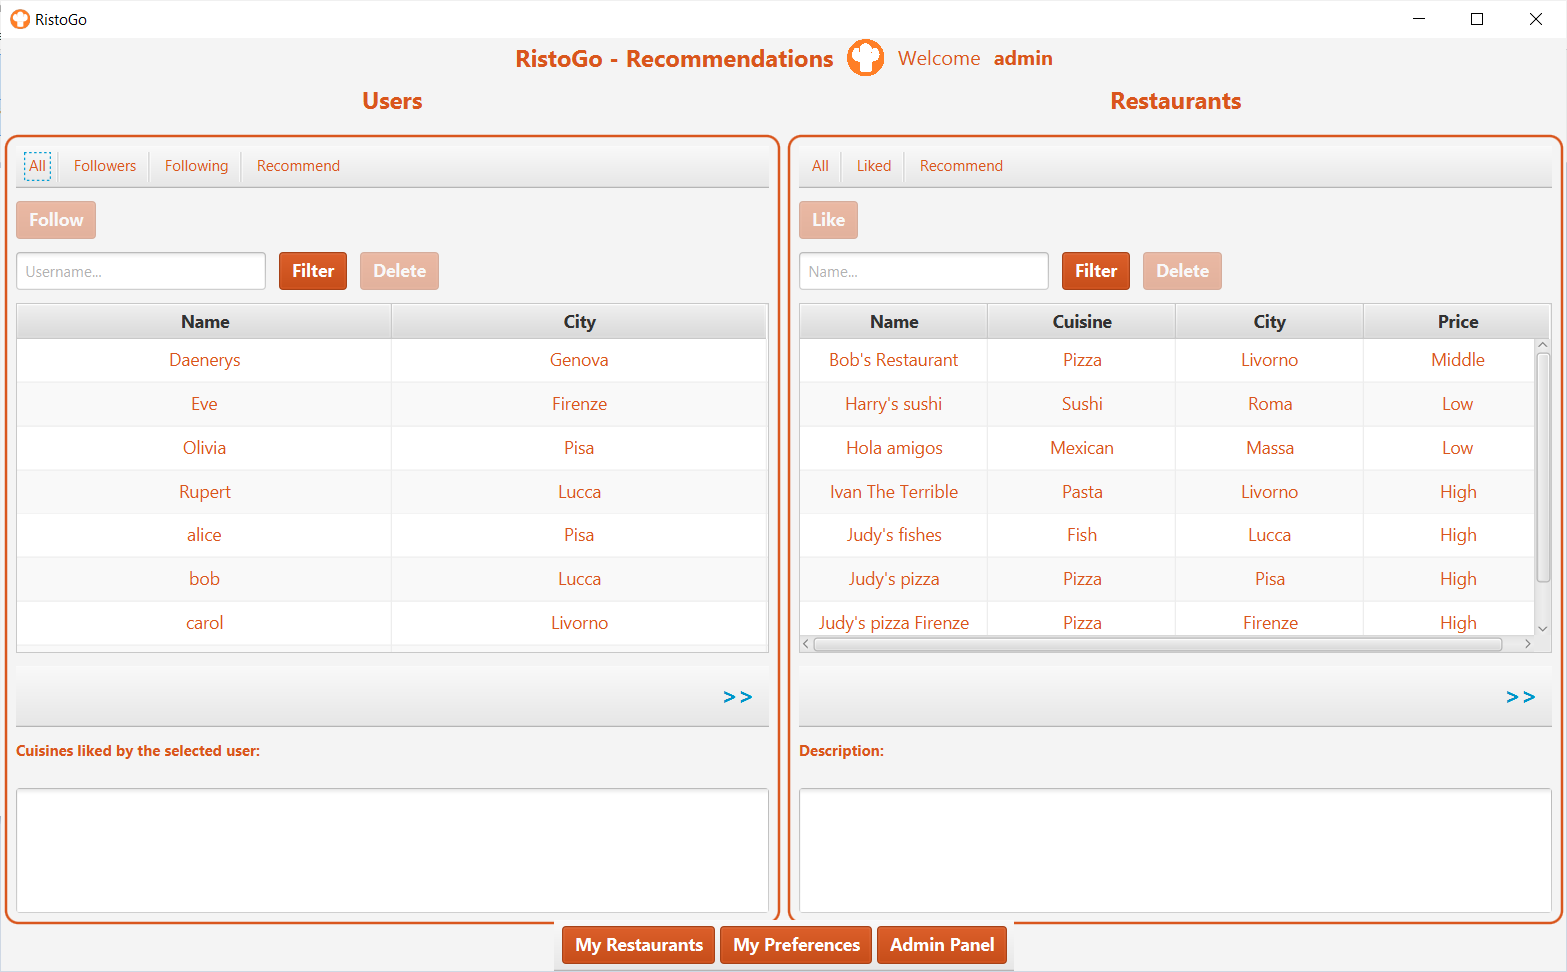
\includegraphics[width=\textwidth]{admin_page}
	\caption{Admin main page.}\label{fig:admin_page}
\end{figure}

\begin{figure}[H]
	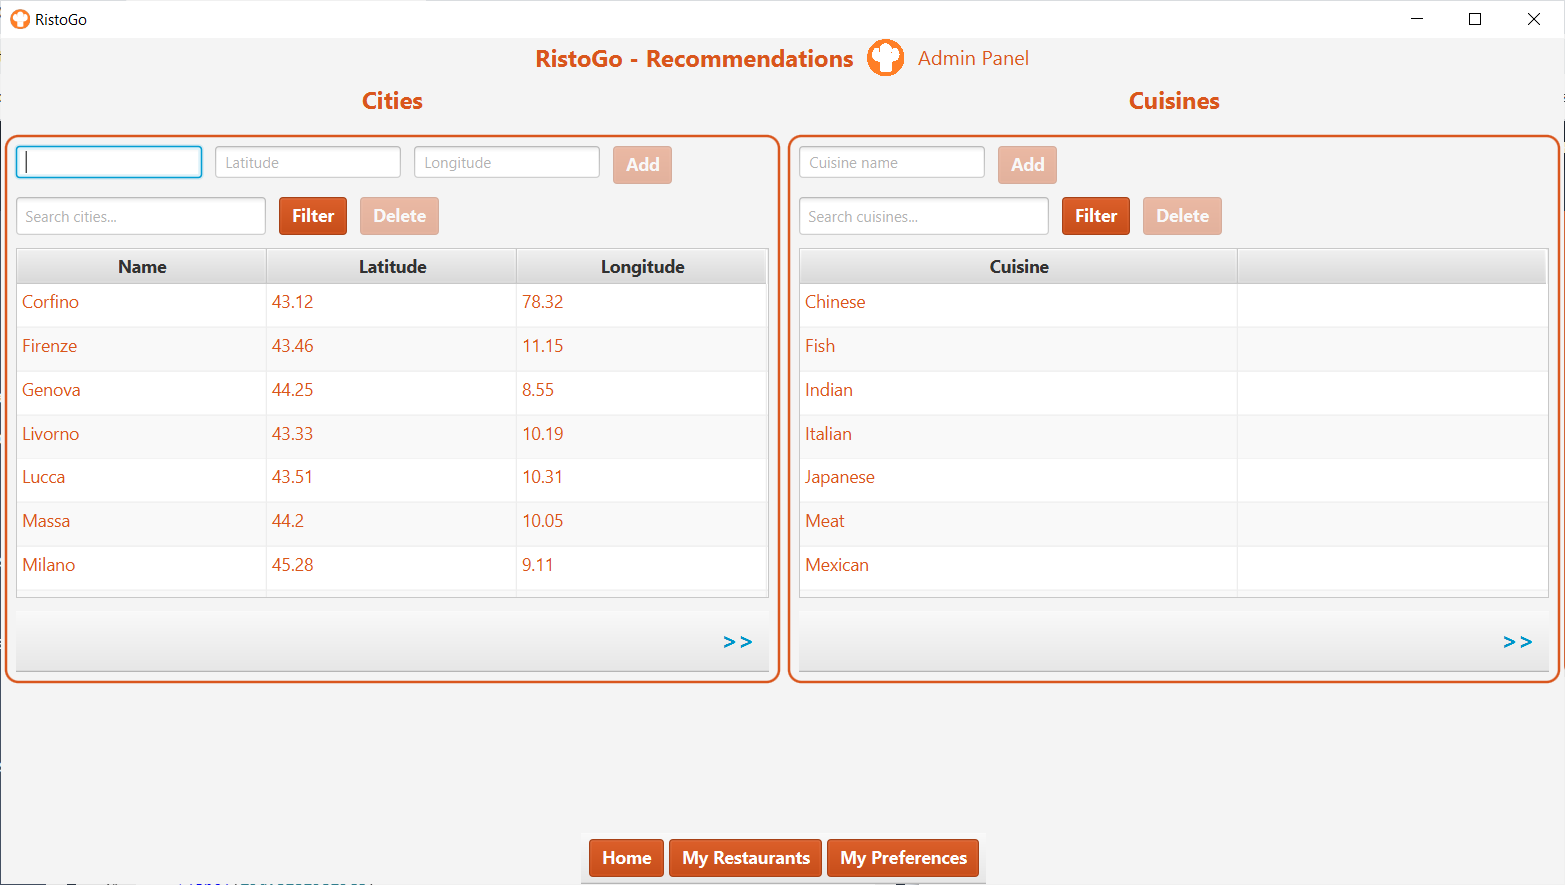
\includegraphics[width=\textwidth]{admin_panel}
	\caption{Admin panel.}\label{fig:admin_panel}
\end{figure}

\subsection{Delete users}

From the list, admin can delete a user selecting it from the list and clicking
on the button ``delete'' (\figref{fig:delete_user}). If there are no errors on
the server, no one can now find that user or his restaurants on the lists.

\begin{figure}[H]
	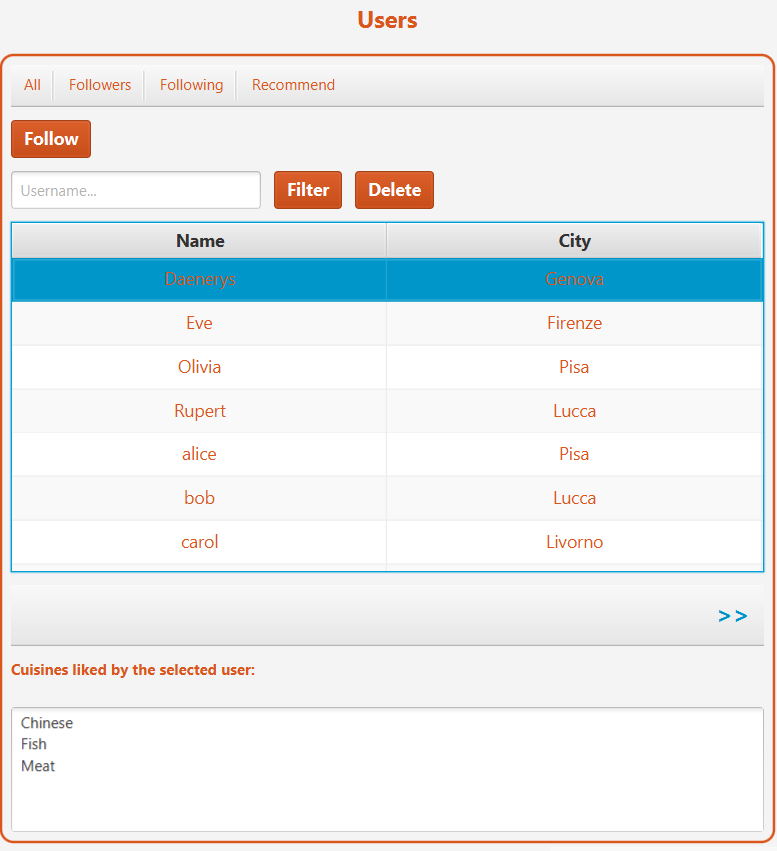
\includegraphics[width=\textwidth]{delete_user}
	\caption{Deleting users.}\label{fig:delete_user}
\end{figure}

\subsection{Delete restaurants}

From the list, admin can delete a user selecting it from the list and clicking
on the button ``delete'' (\figref{fig:delete_restaurants}). If there are no
errors on the server, no one can now find that restaurant on the lists.

\begin{figure}[H]
	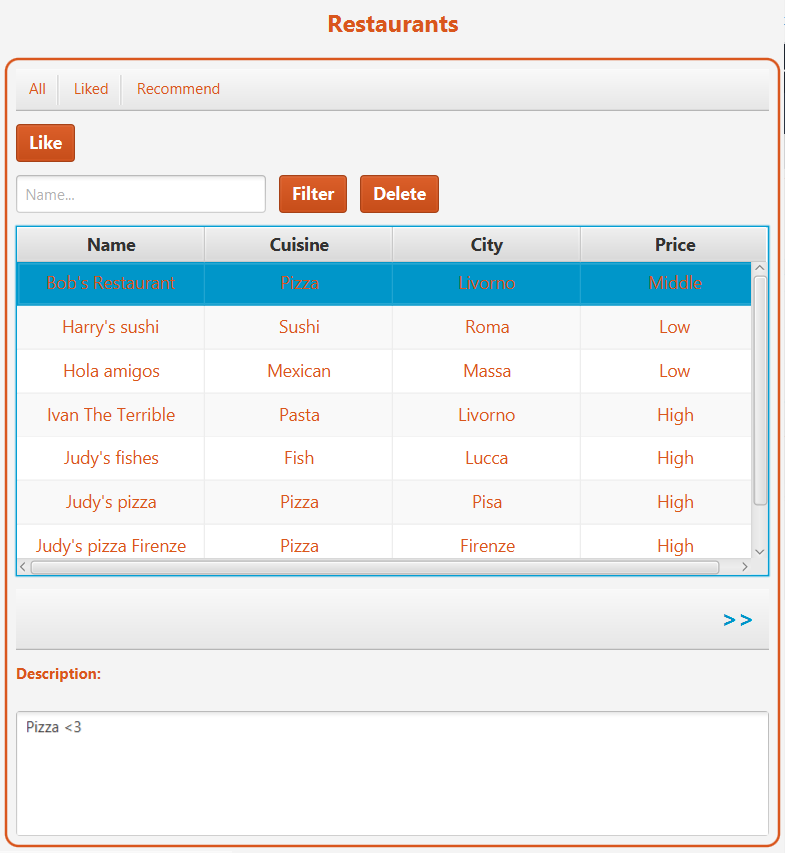
\includegraphics[width=\textwidth]{delete_restaurants}
	\caption{ADeleting restaurants.}\label{fig:delete_restaurants}
\end{figure}

\subsection{Manage cities}

Admin can manage application cities from the admin panel.

He can create a new one inserting its information on the form and then clicking
on ``add'' (\figref{fig:add_city}). If there are no errors you can see the city
on the list (\figref{fig:modify_city}).

He can modify a city selecting it, modifying the parameters and clicking on
``save'' (\figref{fig:modify_city}). If there are no errors you can see the
modified city in the list (\figref{fig:delete_city}).

He can also delete a city selecting it and clicking on the button ``delete''
(\figref{fig:delete_city}). If there are no errors, now the city isn't anymore
on the list and all the users/restaurants located in that city have the city
parameter set to ``N/D''. (\figref{fig:view_city}).

\begin{figure}[H]
	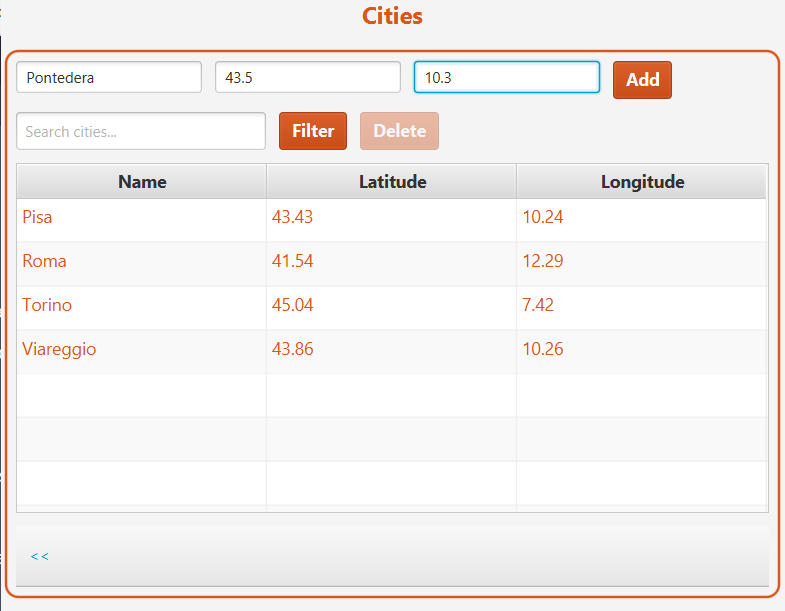
\includegraphics[width=\textwidth]{add_city}
	\caption{Add a new city.}\label{fig:add_city}
\end{figure}

\begin{figure}[H]
	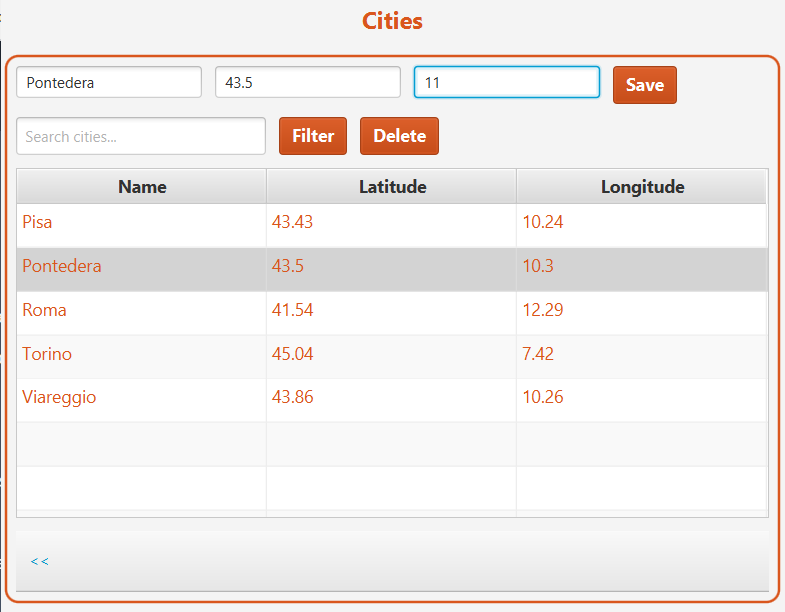
\includegraphics[width=\textwidth]{modify_city}
	\caption{Modify a city.}\label{fig:modify_city}
\end{figure}

\begin{figure}[H]
	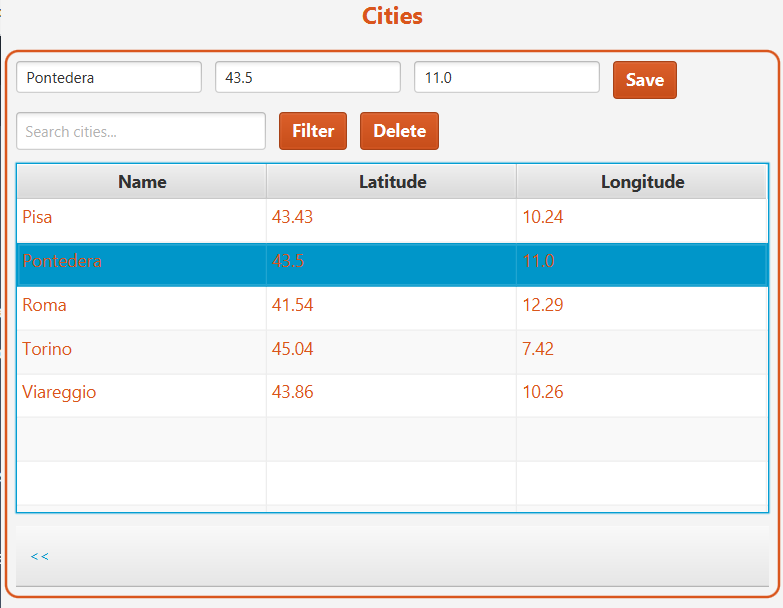
\includegraphics[width=\textwidth]{delete_city}
	\caption{Delete a city.}\label{fig:delete_city}
\end{figure}

\begin{figure}[H]
	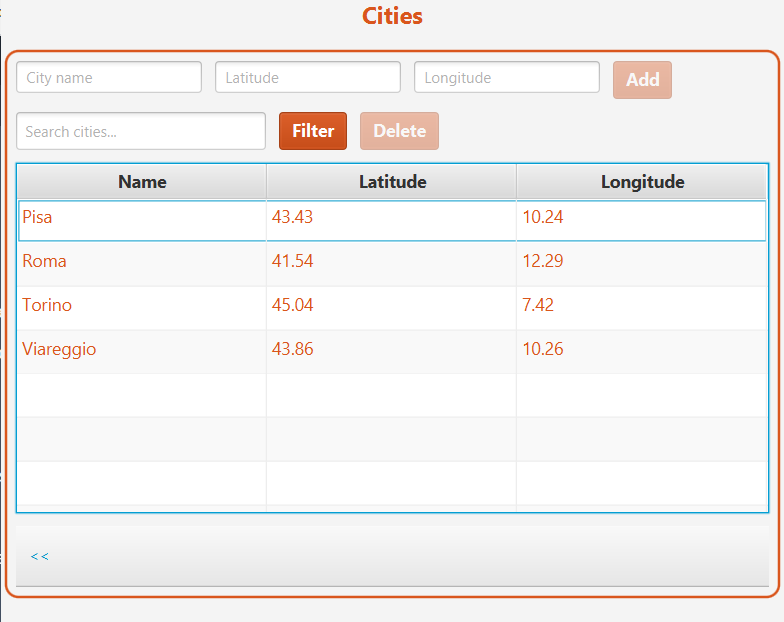
\includegraphics[width=\textwidth]{view_city}
	\caption{List of cities after a delete operation.}\label{fig:view_city}
\end{figure}

\subsection{Manage cuisines}

The same operations of cities can be done also for cuisines, so admin can
create, modify or delete a cuisine, in the same way wrote on the last subsection
(\figref{fig:cuisines}).

\begin{figure}[H]
	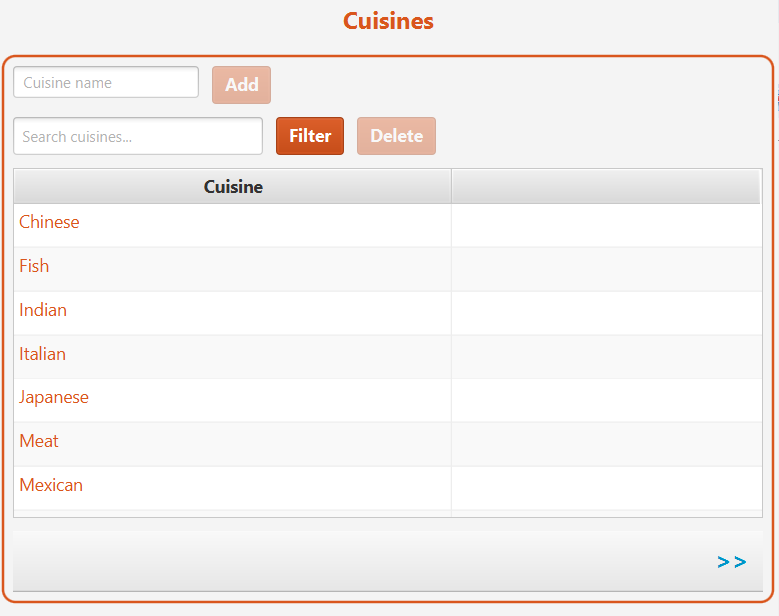
\includegraphics[width=\textwidth]{cuisines}
	\caption{Admin cuisines view.}\label{fig:cuisines}
\end{figure}
